\chapter{$\chi$-boundedness}

\begin{notation}
	$\chi(G) = $ chromatic number $G$ and $\omega(G) = $ is the maximal clique in $G$.
\end{notation}

\begin{observ}
	$\forall G: \chi(G) \geq \omega(G)$.
\end{observ}

\begin{defn}
	Graph class $\mathcal{C}$ is $\chi$-bounded if $\exists f : \N \to \N$ s.t. $\forall G \in \mathcal{C} : \chi(G) \leq f(\omega(G))$.
\end{defn}

\begin{example}
	$\chi$-omezené třídy: úplné grafy, rovinné grafy (funkce $f$ je konstantní), perfektní grafy.
\end{example}

\begin{observ}
	Intervalové, permutační, chordální, comparability, $\dots$ jsou perfektní a tudíž i $\chi$-omezené.
\end{observ}

\section{$\chi$-boundedness of CIRC graphs}

\begin{observ}
	Circular-Arc grafy splňují: $\chi(G) \leq 2 \omega(G)$.
\end{observ}

\begin{proof}
	Na kružnici máme intervaly. V jednom bodě kružnici rozstřihneme a obarvíme $\omega(G)$ barvami. Potom už máme jen intervalový graf, který je perfektní.
\end{proof}

\begin{defn}
	Následující definice jsou si ekvivalentní:
	
	\begin{itemize}
		\item $G \in \text{CIR}$.
		\item $G$ je průnikový graf sečen v kružnici.
		\item $G$ je průnikový graf půlkružnic nad $x$-ovou osou.
		\item $G$ se dá reprezentovat posloupností čísel, kde se každé číslo $1, \dots, n$ vyskytuje právě dvakrát a platí, že vrcholy $v_i, v_j$ spolu sousedí právě když ta posloupnost obsahuje podposloupnost $i,j,i,j$ nebo $j,i,j,i$.
	\end{itemize}
\end{defn}

\begin{thm}
	$\text{CIR}$ je $\chi$-omezená.
\end{thm}

\begin{notation}
	Pro $k \in \N$ definujeme $\text{CIR}(k) := \{G \in \text{CIR}: \omega (G) \leq k\}$.
\end{notation}

\begin{observ}
	$\text{CIR}(k) \subseteq \text{CIR}(k+1) \subseteq \dots \subseteq \text{CIR}$.
\end{observ}

Chceme dokázat, že $(\forall k \in \N) \ (\exists f(k) \in \N) \ : \forall G \in \text{CIR}(k)$ platí, že $\chi(G) \leq f(k)$.

\begin{defn}
	Mějme $G \in \text{CIR}$ reprezentovaný jako průnikový graf půlkružnic. Pro $p,q \in \N_0$ $(p,q)$\textbf{-konfigurace} je množina $p+q$ vrcholů $x_1, \dots, x_p, y_1, \dots, y_q$ takové, že půlkružnice mají tuto vzájemnou polohu zobrazenou na obrázku \ref{konf}.
	
	\begin{figure}[!ht]\centering
		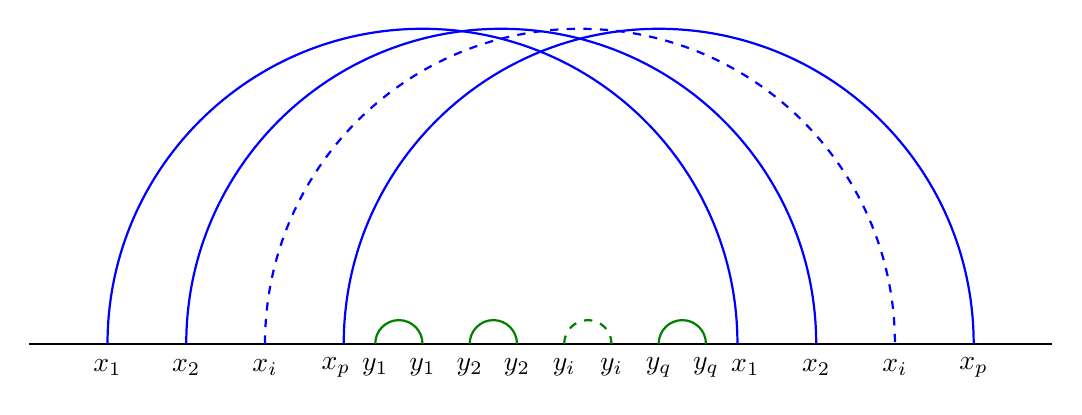
\begin{tikzpicture}
			\draw[thick] (0,0) -- (13,0);
			\draw[color=Blue, thick] (1,0) arc (180:0:4);
			\draw[color=Blue, thick] (2,0) arc (180:0:4);
			\draw[color=Blue, thick, dashed] (3,0) arc (180:0:4);
			\draw[color=Blue, thick] (4,0) arc (180:0:4);
			\draw[color=Green, thick] (4.4,0) arc (180:0:.3);
			\draw[color=Green, thick] (5.6,0) arc (180:0:.3);
			\draw[color=Green, thick, dashed] (6.8,0) arc (180:0:.3);
			\draw[color=Green, thick] (8,0) arc (180:0:.3);
			\node at (1, -.3) {$x_1$};
			\node at (2, -.3) {$x_2$};
			\node at (3, -.3) {$x_i$};
			\node at (3.9, -.3) {$x_p$};
			\node at (4.4, -.3) {$y_1$};
			\node at (5, -.3) {$y_1$};
			\node at (5.6, -.3) {$y_2$};
			\node at (6.2, -.3) {$y_2$};
			\node at (6.8, -.3) {$y_i$};
			\node at (7.4, -.3) {$y_i$};
			\node at (8, -.3) {$y_q$};
			\node at (8.6, -.3) {$y_q$};
			\node at (9.1, -.3) {$x_1$};
			\node at (10, -.3) {$x_2$};
			\node at (11, -.3) {$x_i$};
			\node at (12, -.3) {$x_p$};
		\end{tikzpicture}
		\caption{Definice $(p-q)$-konfigurace.}
		\label{konf}
	\end{figure}
\end{defn}

\begin{notation}
	$\text{CIR}(k,p,q) = \{G \in \text{CIR}, \omega(G) \leq k, G \text{ má reprezentaci bez } (p,q)\text{-konfigurace}\}$.
\end{notation}

\begin{observ}
	Pro $p > k$ a libovolné $q \in \N_0$: $\text{CIR}(k,p,q) = \text{CIR}(k)$.
\end{observ}

\begin{claim}
	$\forall k \in \N \ \forall p, q \in \N_0 \ \exists g(k,p,q) \in \N$ t.ž. $\forall G \in \text{CIR}(k,p,q) : \chi(G) \leq g(k,p,q)$.
\end{claim}

\begin{observ}
	Důkazem tohoto tvrzení platí věta.
\end{observ}

\begin{proof}
	Dané tvrzení dokážeme pomocí dvojité indukce: Indukcí podle $p \in \N_0$:
	
	\begin{lemma}
		$\forall G \in \text{CIR}(k,0,q) : \chi (G) \leq k (q-1)$ pro $q \geq 2$.
	\end{lemma}
	
	\begin{proof}[Proof of lemma]
		Indukcí podle $q \in \N_0$. Pokud $q = 2$ tak můžeme pozorovat, že všechny obloučky protínají společnou souvislou přímku. Tím pádem $\forall k : \text{CIR}(k,0,2) \subseteq \text{PER}$ které jsou perfektní.
		
		Nyní nechť $q > 2$. Nechť $G \in \text{CIR}(k, 0, q)$, vrcholy $G$ rozdělíme na 2 části $V_1, V_2$ tak, že
		
		\begin{itemize}
			\item $V_1$ bude indukovat graf z $\text{CIR}(k,0,2)$ a
			\item $V_2$ bude indukovat graf z $\text{CIR}(k,0,q-1)$.
		\end{itemize}
		
		Označme $\pi$ jakožto nejpravější levý konec obloučku. Potom $V_1$ jsou vrcholy, které mají levý konec vlevo od $\pi$. A $V_2$ jsou vrcholy, které mají levý konec napravo od $\pi$. Pak už použijeme indukci.
	\end{proof}
	
	\begin{lemma}
		Nechť $p \geq 1, q \geq 1$. Potom $\forall G \in \text{CIR}(k,p,q):$ vrcholy $G$ lze rozdělit na 2 části $V_A, V_B$ tak, že každá komponenta $G[V_A]$ i $G[V_B]$ patří do $\text{CIR}(k, p-1, 2q+1)$.
	\end{lemma}
	
	\begin{cor}
		Lze vzít $g(k,p,q) = g (k, p-1, 2q+1)$ tedy tvrzení pak platí.
	\end{cor}
	
	\begin{proof}[Proof of lemma]
		Mějme $G \in \text{CIR}(k,p,q)$. BÚNO: $G$ je souvislý a máme danou repre-\\zentaci. Nechť $x_0$ je vrchol $G$ jehož oblouček má nejlevější levý konec. Definujeme $V_i := \{x \in V(G) : \text{ nejkratší cesta v } G \text{ od } x_0 \text{ do } x \text{ má délku } i\}$.
		
		\begin{observ}
			Pokud vede hrana z $V_i$ do $V_j$ tak $|i - j| \leq 1$.
		\end{observ}
		
		\begin{observ}
			Z každého vrcholu $V_{i+1}$ vede aspoň 1 hrana do $V_i$.
		\end{observ}
		
		Nyní tvrdíme, že žádná komponenta $G[V_i]$ neobsahuje $(p-1, 2q + 1)$-konfiguraci.
		
		Nechť $C$ je komponenta $G[V_i]$ pro spor obsahující $(p-1, 2q + 1)$-konfiguraci. Označme $y_{q+1}$ nějaký oblouček $w$ musí protnout $y_{q+1}$, tedy $w \in V_{i-1}$. Aspoň jeden konec je mimo $C$. $V_{i-1} = V_0$ tedy hotovo. Kdyby měl oba konce v $C$, tak nelze protnout oblouček z $V_{i-2}$.
		
		Nyní nechť $x_1, \dots, x_{p-1}, y_{1}, \dots, y_{2q+1}$ je $(p-1, 2q + 1)$-konfigurace. Nechť $I$ je interval mezi nejlevějším a nejpravějším koncem obloučku v $C$.
		
		\begin{observ}
			Každý soused $w \in V_{i-1}$ vrcholu $y_{q+1}$ musí mít jeden konec mimo $I$.
		\end{observ}
		
		Potom $w, x_1, \dots, x_{p-1}, y_{1}, \dots, y_q$ nebo $w, x_1, \dots, x_{p-1}, y_{q+2}, \dots, y_{2q+1}$ je $(p,q)$-konfi-\\gurace v $G$, což je spor.
		
		Závěrem $V_{A} := \cup_{i \text{ sudé}} V_{i}$ a $V_{B} := \cup_{i \text{ liché}} V_{i}$.
	\end{proof}
\end{proof}

\section{$\chi$-unboundedness of SEG graphs}

\begin{defn}
	SEG is the class of graphs of intersection graphs of segments in the plane.
\end{defn}

Now the question might be if SEG graphs are $\chi$-bounded or not. This was firstly stated by Erdos. The answer came later by the following theorem.

\begin{thm}[Pawlik, Kozik, Krawczyk, Lagos, Micek, Trotter, Wolezak, 2012]
	$\forall k \in \N$ there exists triangle-free graph $G_k \in \text{SEG}$ with $\chi(G_k) \geq k$.
	\label{PKKLMTW thm}
\end{thm}

\begin{defn}
	\textbf{L-curve} is a union of a horizontal and vertical segment sharing a common bottom-left endpoint. \textbf{L-graph} is an intersection graph of L-curves.
\end{defn}

\begin{thm}
	Any L-graph is also SEG-graph.
\end{thm}

\begin{proof}
	Suppose $\mathcal{L} = \{l_1, l_2, \dots, l_n\}$ is a set of L-curves, we will show by induction on $\abs{\mathcal{L}} = n$ that there is a set $\mathcal{S} = \{s_1, s_2, \dots, s_n\}$ of segments s.t. $l_i \cap l_j \neq \emptyset \Leftrightarrow s_i \cap s_j \neq \emptyset$, and moreover:
	
	\begin{enumerate}
		\item all $s_1, \dots, s_n$ lie in the half plane below the $x$-axis;
		\item $s_i$ touches the $x$-axis \ifft $l_i$ can be extended upwards to infinity without crossing any other $l_j \in \mathcal{L}$;
		\item left-to-right order of $s_i$'s touching the $x$-axis is the same as for $l_i$'s.
	\end{enumerate}
	
	Now for $n = 1$ it is simple, see Fig. \ref{}, and for $n > 1$ WLOG $l_n$ has topmost horizontal part. By induction we represent $\mathcal{L}' = \{l_1, \dots, l_{n-1}\}$ by $\mathcal{S}' = \{s_1, \dots, s_{n-1}\}$ then
	
	\begin{enumerate}
		\item shorten the $s_i$ if $l_i$ no longer can extend upwards and
		\item insert $s_n$ touching $x$-axis, nearly horizontal. See Fig. \ref{}.
	\end{enumerate}
	\begin{figure}[!ht]\centering
		\caption{Proof examples.}
	\end{figure}
\end{proof}

\begin{proof}[Proof of theorem \ref{PKKLMTW thm}]
	In fact we show that $\forall k \in \N$ there exists triangle-free L-graph $G_k$ with $\chi(G_k) \geq k$.
	
	\begin{defn}
		A \textit{configuration} is
		
		\begin{enumerate}
			\item a collection of L-curves inside the unit square $[0,1] \times [0,1]$, whose intersection graph os triangle-free
			\item a set $\{P_1, \dots, P_m\}$ of \textit{"probes"} which are pairwise disjoint rectangles inside $[0,1] \times [0,1]$ touching its bottom boundary
			\item any L-shape from the collection intersecting a probe $P_i$ must cross it from left to right
			\item the L-shape crossing a given probe are pairwise disjoint.
		\end{enumerate}
		
		\begin{figure}[!ht]\centering
			\caption{Example of definition.}
		\end{figure}
	\end{defn}
	
	We will construct two sequences of $A_1, A_2, A_3, \dots$ and $B_1, B_2, B_3, \dots$ of configurations s.t.:
	
	\begin{enumerate}
		\item $\forall k \in \N$ in any proper coloring of the L-curves in $A_k$, the L-curves seen inside the probes use at least $k$-different colors.
		\item $\forall k \in \N$ in any proper coloring of the L-curves in $B_k$ there exist a probe of $B_k$ which is crossed by L-curves of at least $k$ different colors.
	\end{enumerate}
	
	By induction for $k = 1$ it is straightforward, see Fig. \ref{}. Now we show two parts.
	
	\begin{figure}[!ht]\centering
		\caption{Figure}
	\end{figure}
	
	\begin{enumerate}
		\item From $B_k$ to $A_k+1$. See Fig. \ref{}.
		\begin{enumerate}
			\item Insert one new L-shape inside every probe of $B_k$ and
			\item replace each probe by 2 new probes.
		\end{enumerate}
		\item From $B_k$ and $A_{k+1}$ to $B_{k+1}$. See Fig. \ref{}.
		\begin{enumerate}
			\item Insert a small copy of $A_{k+1}$ near the top of every probe of $B_k$ and
			\item extend the probes of these small copies all the way down to obtain probes of $B_{k+1}$.
		\end{enumerate}
	\end{enumerate}
	
	\begin{figure}[!ht]\centering
		\caption{Figure}
	\end{figure}
	
	\begin{figure}[!ht]\centering
		\caption{Figure}
	\end{figure}
\end{proof}

Now we may ask ourselves if this prove can be extended to some other type of intersection graphs. Well indeed it can be done. Note that \textit{arc-connected} set means that all pairs from the set can be connected via an arc.

\begin{fact}
	For any compact arc-connected set $X \subseteq \R^2$ other then an axis parallel rectangle there is a triangle-free graph $G_k$, $\chi(G_k) \geq k$, which is the intersection graph of horizontally and vertically scaled copies of $X$.
\end{fact}

\begin{thm}[Asblund, Grunbaum]
	If $G$ is an intersection graph of axis parallel rect-\\angles in the plane then $\chi(G) \leq O(\omega^2 (G))$.
\end{thm}

\begin{proof}
	Suppose we have $G = (V,E)$ as above: each vertex $u \in V$ is represented by a rectangle $R_u$. Let $E = E_1 \dot{\cup} E_2$ as follows
	
	\begin{enumerate}
		\item $\{u,v\} \in E_1$ if a vertex of $R_u$ is inside $R_v$ or vice versa
		\item $E_2 = E \setminus E_1$ if it is cross-like.
	\end{enumerate}
	
	\begin{figure}[!ht]\centering
		\caption{Figure}
	\end{figure}
	
	Lets denote $G_1 = (V, E_1)$, $G_2 = (V, E_2)$ and $k = \omega(G)$. We will show $\chi(G_1) = O(k)$ and $\chi(G_2) = O(k)$.
	
	\begin{itemize}
		\item For $G_1$ we claim that $|E_1| \leq 8 k \cdot |V|$ (and any subgraph of $G_1$ induced by $W \subseteq V$ has at most $8 k \cdot |V|$ edges). This is because each vertex of a rectangle is inside at most $K-1$ other rectangles, due to the maximal clique. Now we direct an edge $uv$ if $R_u$ is inside $R_v$. Thus the outdegree of any vertex is $\leq 4 (k-1)$ so $|E-1| \leq 4 (k-1) \cdot |V|$. Hence $G_1$ (and any of its induced subgraphs) has a vertex of degree $\leq 8 (k-1) \Rightarrow \chi(G_1) \leq 8 (k-1) + 1$.
		\item For $G_2$ we claim that $\chi(G_2) = \omega(G_2) = O(k)$ because $G_@$ is a comparability graph (for example sort the boxes from tallest to shortest).
		\item For $G$ we have $\chi(G) \leq \chi(G_1) \chi(G_2) = O(k^2)$.
	\end{itemize}
\end{proof}